\documentclass[conference]{IEEEtran}
\IEEEoverridecommandlockouts{}
\usepackage{cite}

\usepackage{amsmath,amssymb,amsfonts}
\usepackage{algorithmic}
\usepackage{graphicx}
\usepackage{textcomp}
\usepackage{xcolor}
\usepackage{lipsum}
\definecolor{codegray}{gray}{0.9}
\newcommand{\code}[1]{\colorbox{codegray}{\texttt{#1}}}
\usepackage{fancyvrb} % for "\Verb" macro
\VerbatimFootnotes

\def\BibTeX{{\rm B\kern-.05em{\sc i\kern-.025em b}\kern-.08em


    T\kern-.1667em\lower.7ex\hbox{E}\kern-.125emX}}


\begin{document}

\title{Big Data IU-S25 Assignment 2}

\author{\IEEEauthorblockN{Vsevolod Klyushev}
    \IEEEauthorblockA{\textit{Innopolis University} \\
        Innopolis, Russia \\
        v.klyushev@innopolis.university}
}

\maketitle

\begin{abstract}

In this assignment, we were required to provide an e-commerce solution for a company to store, receive, and analyze information more efficiently. The main objectives were to implement SQL and noSQL data models for an e-commerce company and analyze its performance. I have developed data storage models for databases such as PostgreSQL, MongoDB, and Neo4j and wrote scripts to migrate from the current solution (storing information in csv files) to them.

\end{abstract}

\section{Data Modeling}

\subsection{Data analysis}

The first step to develop a solution is to understand the structure of the data with which we are working. In total, we have 5 files with information about companies, messages, users, events, and connections between users. Based on the information from these tables, I decided to factor out new data objects and remove/reallocate several features. Let us consider them one by one:

\subsubsection{Messages}

This table initially has 34 features, however, not all of them are necessary connected to them. I took the following actions to improve it:
\begin{itemize}
    \item I dropped column \code{category}, since it contained only null values and we had no information about its meaning in the assignment description.
    \item I dropped column \code{id}, since we already have uuid in column \code{message\_id}.
    \item \code{user\_id}, \code{user\_device\_id} and \code{email\_provider} depends on \code{client\_id} and should be moved from \code{messages} table to \code{clients} (also known as \code{client\_first\_purchase\_date} table)
\end{itemize}

\subsubsection{Events}

This is the second table that requires splitting. Feature \code{brand} solely depends on \code{product\_id} and feature \code{category\_code} on \code{price}. With this information, we can create two more tables \code{products} and \code{categories} that would store such dependencies and allow us to remove two unnecessary columns from the table \code{events}.
\\

Such actions for both \code{messages} and \code{events} initial tables helped us to reduce the amount of stored information.

\subsection{Data preprocessing}

The provided data was in very bad shape and required a number of actions to make it better:
\begin{itemize}
    \item In \code{campaigns} table we had to convert float values to int once for columns \code{total\_count}, \code{hour\_limit}, \code{subject\_length} and \code{position}.
    \item Also in \code{campaigns} table feature \code{ab\_test} contained only values \code{null} or \code{True}, thus, we had to convert this nulls to False.
    \item In \code{messages} table columns \code{is\_opened}, \code{is\_clicked}, \code{is\_unsubscribed}, \code{is\_hard\_bounced}, \code{is\_soft\_bounced}, \code{is\_complained}, \code{is\_blocked}, \code{is\_purchased} contained values \code{t} and \code{f}, which had to be substituted with \code{True} and \code{False}.
\end{itemize}

In this section, we can also mention processes such as creating new tables in a way that does not lose data and removes all duplicates or substitutes null values if there is an opportunity.

At the end, we had 7 tables: \code{campaigns}, \code{messages}, \code{clients}, \code{friends}, \code{events}, \code{products} and \code{categories} to work with. All data models would have similar structure based on this tables.

\subsection{PostgreSQL}

\begin{figure}
  \centering
    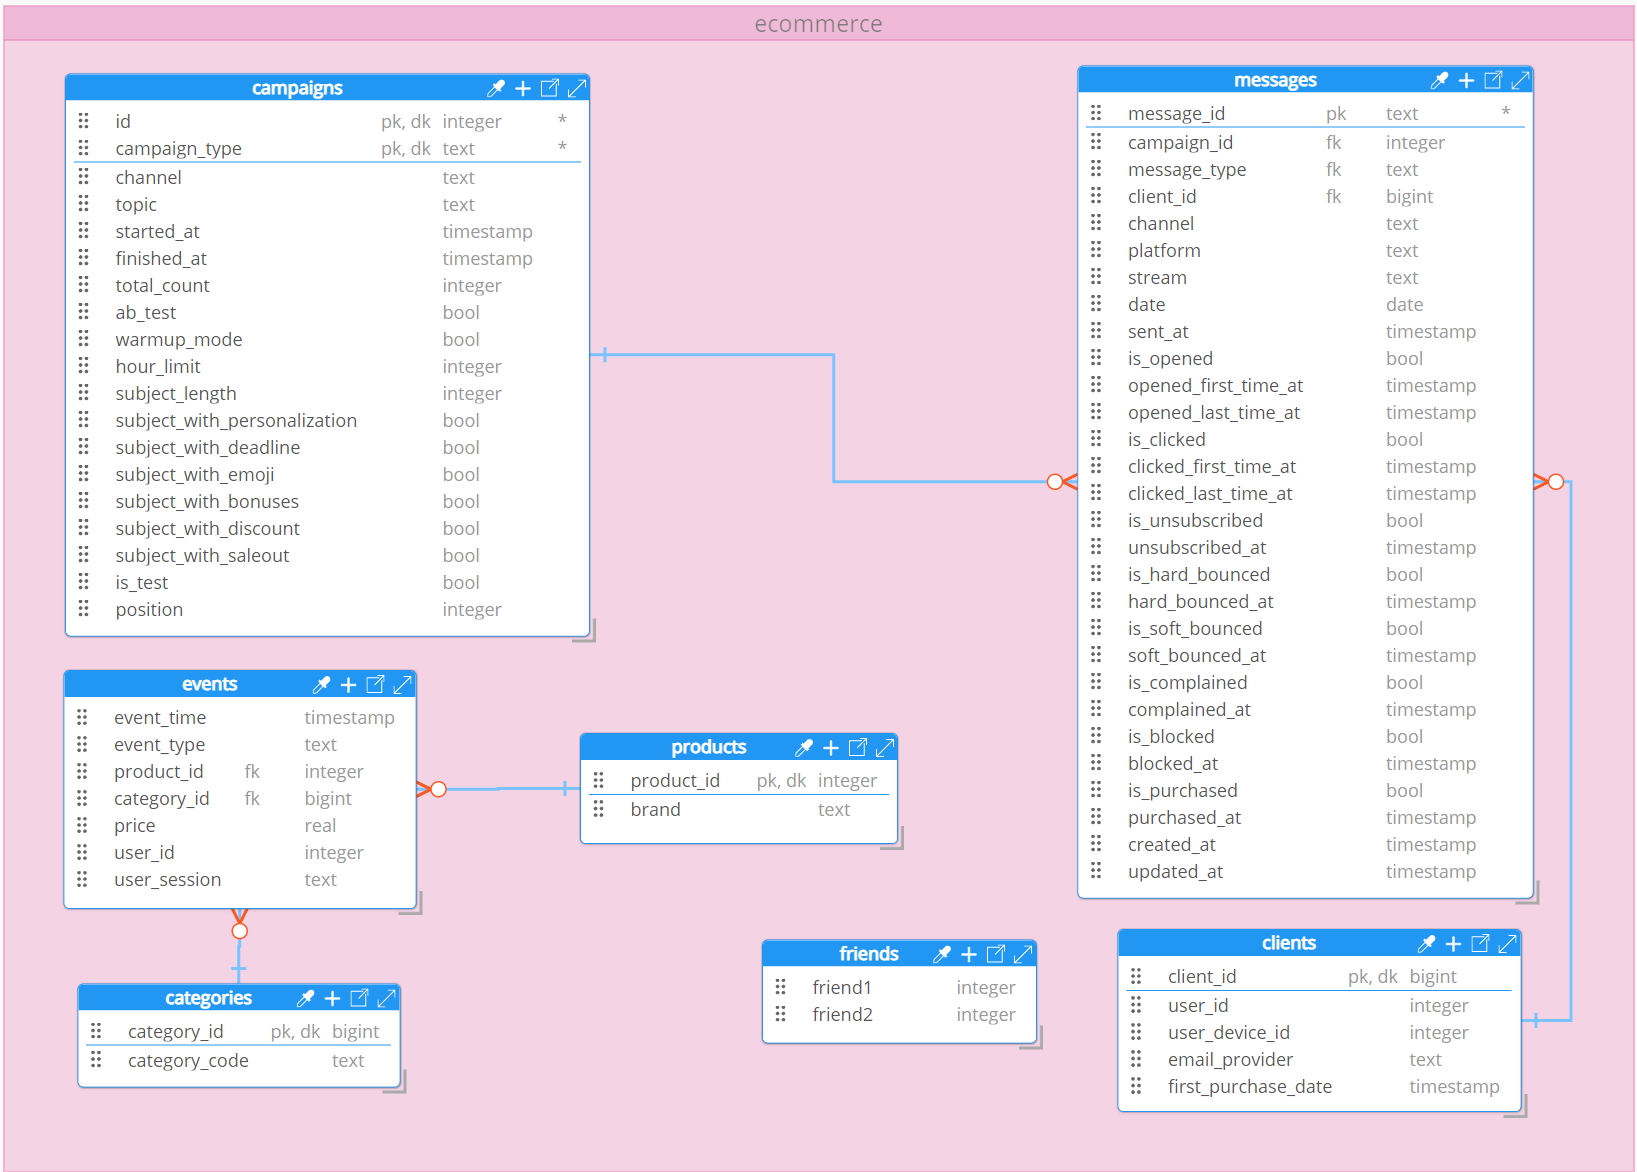
\includegraphics[width=0.5\textwidth]{./pictures/postgres.png}
    \caption[PostgreSQL model]{PostgreSQL model}\label{fig:postgres}
\end{figure}

 Fig. \ref{fig:postgres} contains general structure for PostgreSQL data model. To build an optimal database in postgres, it is necessary to determine the keys and relationships between the tables. Let's start with primary keys:
 \begin{itemize}
     \item Table \code{campaigns} has composite key based on columns \code{id} and \code{campaign\_type}.
     \item Table \code{messages} has primary key \code{message\_id}.
     \item Table \code{clients} has primary key \code{client\_id}.
     \item Table \code{products} has primary key \code{products\_id}.
     \item Table \code{categories} has primary key \code{categories\_id}.
 \end{itemize}

Based on that primary keys we can define foreign keys show connections between tables:
\begin{itemize}
    \item For table \code{messages} fields \code{campaign\_id} and \code{message\_type} are fk which are connected to table \code{campaigns}.
    \item For table \code{messages} field \code{client\_id} is a fk which are connected to table \code{clients}.
    \item For table \code{products} field \code{product\_id} is a fk which are connected to table \code{events}.
    \item For table \code{categories} field \code{category\_id} is a fk which are connected to table \code{events}.
\end{itemize}

After that we can import our preprocessed data from csv files in the PostgreSQL.

\subsection{MongoDB}

\begin{figure}
  \centering
    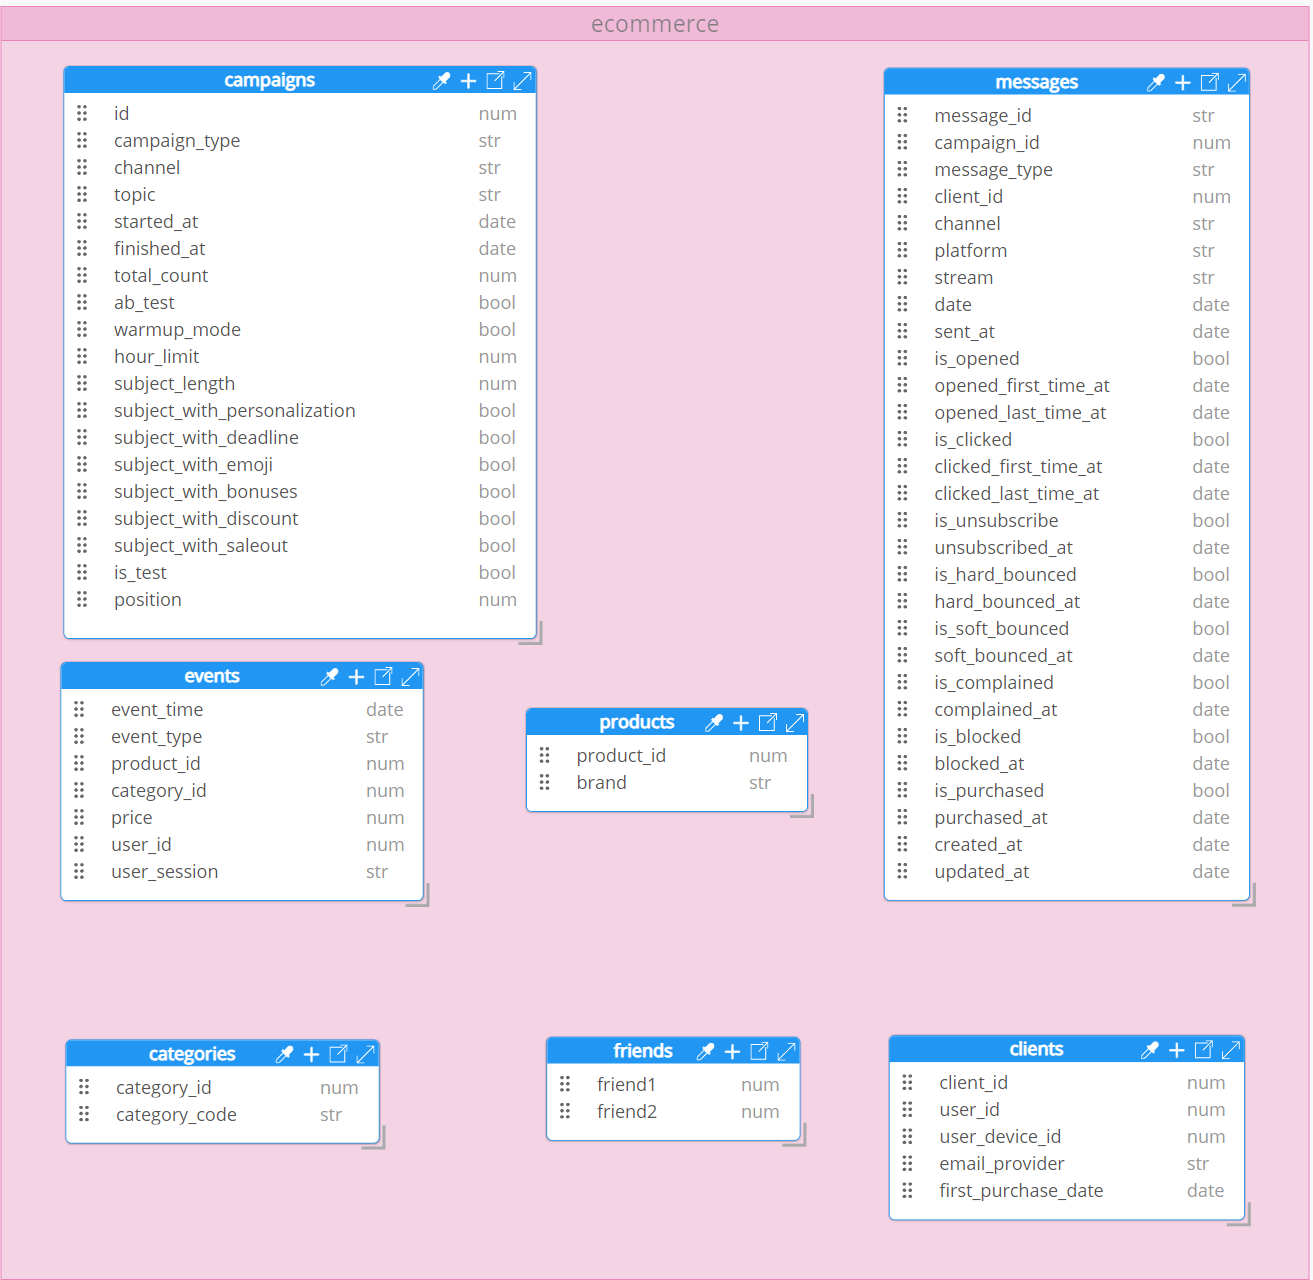
\includegraphics[width=0.5\textwidth]{./pictures/MongoDB.png}
    \caption[MongoDB model]{MongoDB model}\label{fig:mongo}
\end{figure}

 Fig. \ref{fig:mongo} contains general structure for MongoDB data model. As you can see, it's almost the same as in PostgreSQL. However, we faces with several difficulties on importing stage for this noSQL database. First of all, we had to build json files, since MongoDB can't determine that the provided boolean or datetime field is not a string. Even though, we have to rebuild our jsons and manually set for all timestamp fields value in format of \code{\$date: \%Y-\%m-\%dT\%H:\%M:\%SZ} and convert each of them in corresponding time format.

 \subsection{Neo4j}

\begin{figure}
  \centering
    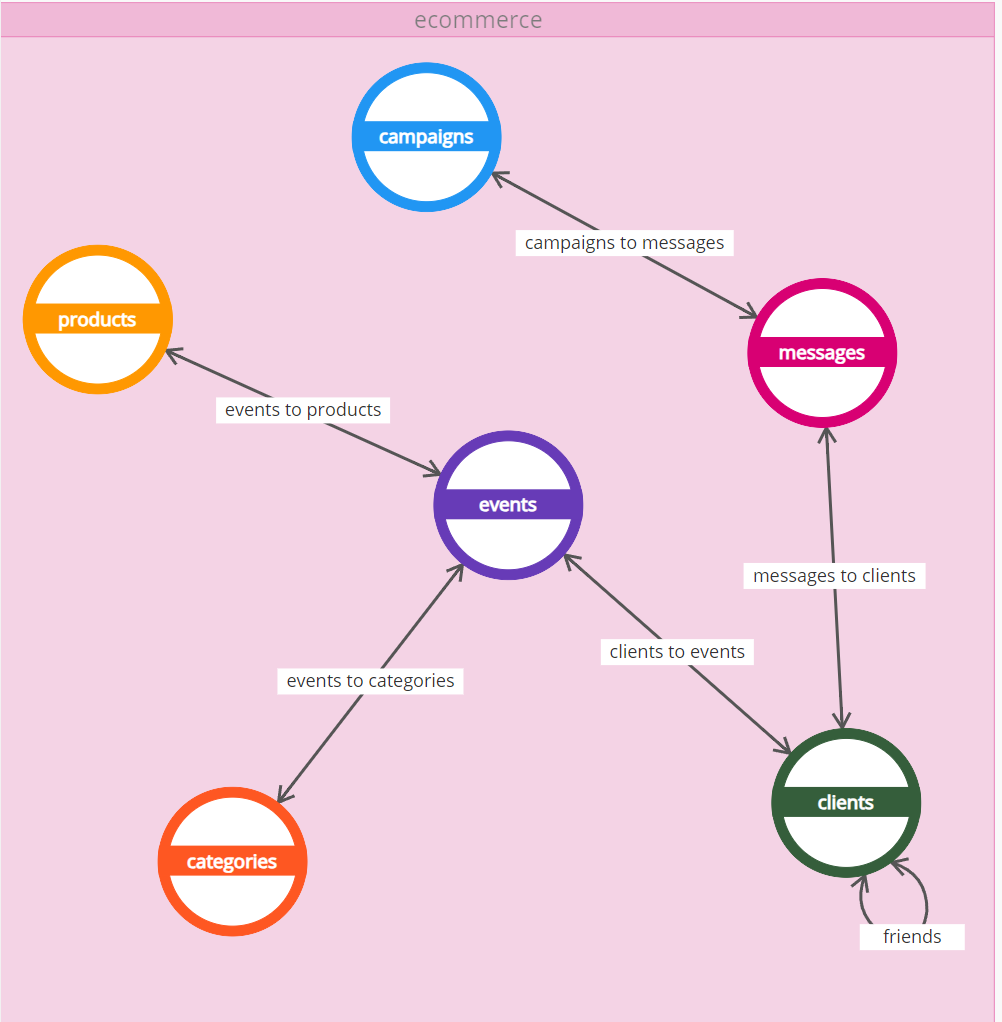
\includegraphics[width=0.5\textwidth]{./pictures/Neo4j.png}
    \caption[Neo4j model]{Neo4j model}\label{fig:neo}
\end{figure}

 Fig. \ref{fig:neo} contains general structure for Neo4j data model, which differs only in putting information from \code{friends} table into relationship between clients. As for connection between nodes, it's very similar to one in PostgreSQL (f.e. \code{messages} connected with \code{clients} nodes via \code{client\_id} property and etc.), however, apart from connection between \code{clients} node via \code{user\_id} field, there is also a new connection from \code{events} to \code{clients} via \code{user\_id field}.

 I want to highlight the importance of indexes for Neo4j fields which are used to build relationships. Without them importing process requires numerous amount of time.

 Also, to import all the data, I had to modify neo4j.conf file to increase memory limits for executions.

\section{Discussion}
I successfully created data models for PostgreSQL, MongoDB and Neo4j databases and imported data in them.
Unfortunately, I did not have time to compare the effectiveness of these models on different queries. It took too long to prepare the environment, models, data, and import data into the databases themselves. Due to the large amount of data in the source files, processing required significant computing resources. Moreover, one error could lead to a long wait for new data to be prepared or uploaded. In addition, it was by no means easy to find a way to correctly import a date from various formats into MongoDB. If there was less data, at least we wouldn't have to wait so long for it to be processed. My opinion is that this assignment requires too much time and efforts for the amount points that it can give.

\section*{Acknowledgment}

The style of this report is inspired by the~\cite{uzunbayir}.

\begin{thebibliography}{00}

    \bibitem{uzunbayir} Serhat Uzunbayir. Relational database and nosql inspections using mongodb and neo4j on a big data application.

    In 2022 7th International Conference on Computer Science and Engineering (UBMK), pages 148--153, 2022.

    doi:10.1109/UBMK55850.2022.9919589.

\end{thebibliography}

\end{document}

